\documentclass[10pt,letterpaper]{article}
\usepackage[utf8]{inputenc}
\usepackage{amsmath}
\usepackage{amsfonts}
\usepackage{amssymb}
\usepackage{graphicx}
\usepackage[left=1in,right=1in,top=1in,bottom=1in]{geometry}

\usepackage{subfig}
\usepackage{xcolor}
\newcommand{\cbox}[1]{\raisebox{2pt}{\fcolorbox{black}{#1}{\null}}}

\definecolor{blueplot}{HTML}{1f77b4}
\definecolor{orangeplot}{HTML}{ff7f0e}

\usepackage{tikz, pgf}
\usetikzlibrary{automata, positioning, arrows}

\title{Thesis Corrections}
\author{Max Bremer}

\begin{document}
\maketitle

\subsection*{Abstract}
Here is an overview of the answers to each question. The questions are answered extensively in their respective sections. At the start of each section, I have also included italicized information describing the location of edits in the thesis.
\begin{itemize}
\item {\bf Quantify the amount of misspeculation:} The overall amount of misspeculation is relatively low ($\le 5\%$) of non-trivial updates. For the Carrier-Greenspan problem, misspeculation occurs near regions where the timestep is changing. For the lake at rest problem, it occurs near regions certain regions where there are large discrepancies in the amount of per actor work. To assess the impact of misspeculation on the time to solution, we use an integrated imbalance metric to determine when roll back is occurring on the critical path. For the Carrier-Greenspan problem, we found relatively  little impact on time to solution due to misspeculation, and for the polynomial mesh lake at rest, we estimate the time to solution could be accelerated by $12\%$ through the elimination of bad speculation.
\item {\bf Justify better why you did not explore conservative event-driven simulation:} Deriving good look ahead estimates for the local timestepping algorithm is very difficult. Without good look ahead estimates, we expect there to be insufficient parallelism to ensure good parallel performance. Furthermore, given the good performance of the optimistic PDES implementation, we believe a good use case is required to justify the development of a conservative parallelization.
\item {\bf Give an estimate of how much time partitioning takes:} For the load balancing portion of the thesis, mesh repartitioning takes between $700 \mathrm{ms}$ to $3700 \mathrm{ms}$ based on the number of submeshes and nodes being simulated. For the adaptive local timestepping problem, partitioning takes 6 minutes using Gurobi, and the incumbent best simulation is used at the end of partitioning. However, this partitioning strategy is not a viable strategy in general, and deriving better load balancing schemes is a topic of ongoing work.
\end{itemize}

\subsubsection*{Quantify the amount of misspeculation.}
{\it This section has been added as section starting on p. 95}

\begin{figure}
\centering
\subfloat[Lake at Rest--Uniform\label{fig:rb:actor:lar:uniform}]{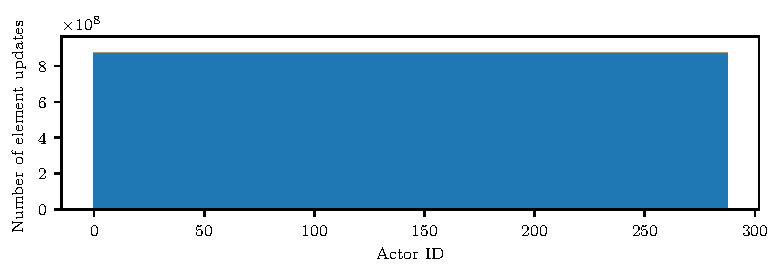
\includegraphics{images/lake_at_rest_uniform_actor_work}}\\
\subfloat[Lake at Rest--Polynomial\label{fig:rb:actor:lar:polynomial}]{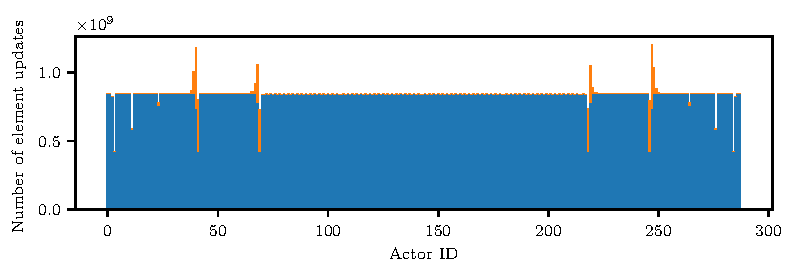
\includegraphics{images/lake_at_rest_polynomial_actor_work}}\\
\subfloat[Carrier-Greenspan--Uniform
\label{fig:rb:actor:cg:uniform}]{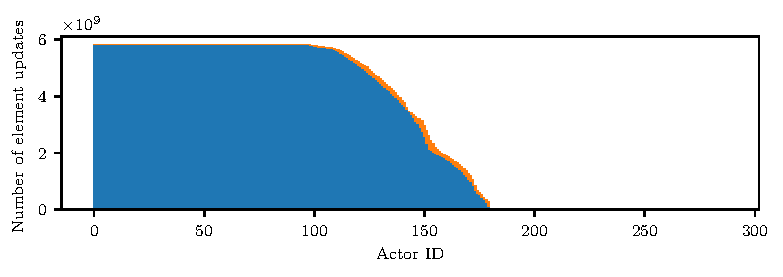
\includegraphics{images/carrier_greenspan_uniform_actor_work}}\\
\subfloat[Carrier-Greenspan--Polynomial\label{fig:rb:actor:cg:polynomial}]{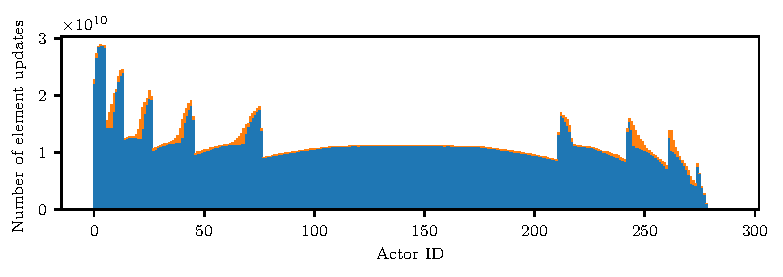
\includegraphics{images/carrier_greenspan_polynomial_actor_work}}
\caption{Cumulative number of element updates committed---shown in \cbox{blueplot}---and rolled back---shown in \cbox{orangeplot} updates for each actor.}
\label{fig:rb:actor}
\end{figure}

Since we are able to make updates arbitrarily expensive through the addition of cells to a submesh in order to hide task overheads, we only look at rollbacks of non-trivial updates. Events such as push fluxes or updates for which $\lceil t \rceil$ does not match the current simulation time, require little work and rolling them back incurs relatively little overhead.
To help understand the behavior of rollback for the simulation, we plot the total number of elements updated and rolled-back per {\em actor} in Figure~\ref{fig:rb:actor}. Since all considered problems are one dimensional, the actors are ordered to reflect their positions in the mesh, i.e. actor 0 updates the leftmost submesh, and actor 1 corresponds to the submesh immediately to the right of the leftmost submesh, etc.
We also plot the commits and rollbacks performed by each {\em rank} in Figure~\ref{fig:rb:rank}. For the lake at rest problem, ranks are assigned 6 contiguous actors. Hence, similar to the actors, the rank ID corresponds to the position relative to other ranks. However, for the Carrier-Greenspan problem, the integer programming problem does not consider submesh locality and any rank may be assigned submeshes from anywhere in the mesh.


 For the lake at rest problem on either of the two meshes, shown in Figure \ref{fig:rb:actor:lar:uniform} and \ref{fig:rb:actor:lar:polynomial}, we see that the partitioning strategy creates submeshes which require roughly the same amount of work to update. The partitioning into submeshes assumes no knowledge of the wave speed $\Lambda$ and thus uses $|\Lambda|\equiv 1$. Since this corresponds exactly to the $|\Lambda|$ of the lake at rest problem, we achieve a good distribution of work between actors. In Figure \ref{fig:rb:actor:lar:polynomial}, we note that a few submeshes are assigned significantly less work than the mean amount of work. This arises due to the non-uniform increments in work added by a single cell. In the iterative submesh partitioning process, if a cell which is constraining the CFL condition for a submesh is removed from that submesh, the submesh will take a larger timestep, thus lowering the overall amount of work associated with that given submesh. Figure~\ref{fig:rb:actor:lar:polynomial} shows that near these under worked regions is also where rollback occurs. As seen in Figure~\ref{fig:rb:rank:lar:polynomial}, the ranks which contain these submeshes are assigned less work yet incur significant rollback. Ultimately this speculation causes these ranks to perform the largest number of element updates and determine the critical path of the simulation.
 
For the Lake at Rest-Uniform configuration shown in Figure~\ref{fig:rb:actor:lar:uniform}, the submesh detects stutter stepping after each update and waits. In this case, no updates are rolled back, and due to the balanced submesh partitioning, the imbalance is negligible.


For the Carrier-Greenspan problem, we observe that not all submeshes are assigned the same amount of total work, since the flow field is not constant. For the uniform mesh shown in Figure~\ref{fig:rb:actor:cg:uniform}, we note that the number of updates per actor is relatively similar for the left side of the mesh. In the center of the mesh, the cells are wetting and drying as the oscillatory wave passes over them. 
There is a small amount of rollback occurring, and updates per actor decrease as the water gets shallower. The right portion of the mesh, which does not execute any updates. The Carrier-Greenspan problem on the polynomial mesh heavily distorts the center of submesh. The sharply spiked pattern corresponds to timestep transition regions. The total rollback for both meshes remains low overall, with $1.3\%$ of element updates being rolled back for the uniform mesh and $3.4\%$ of element updates being rolled back for the polynomial mesh. 

\begin{figure}
\centering
\subfloat[Predicted $\Delta t$]{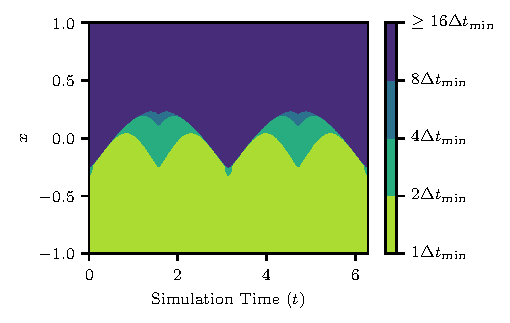
\includegraphics{images/theoretical_dt}}
\subfloat[Observed Rollback]{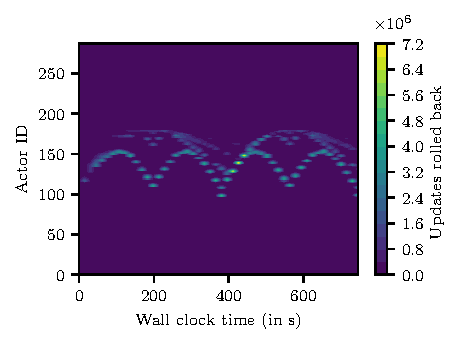
\includegraphics{images/rollback_temporal}}
\caption{Temporal occurrence of rollback compared to expected timestep size for the Carrier-Greenspan problem on the uniform mesh.}
\label{fig:rb:temporal}
\end{figure}

In Figure~\ref{fig:rb:temporal}, we compare the theoretical timestep size based on the analytic solution against the time-resolved location of rollback for the Carrier-Greenspan problem on the uniform mesh. Rollback in this case tends to only occur near regions where the timestep is changing. At any given point, only a very small number of updates are rolled-back. However, the location of roll-back depends on the solution and therefore cannot be known a priori in general.


\begin{figure}
\centering
\subfloat[Lake at Rest--Uniform]{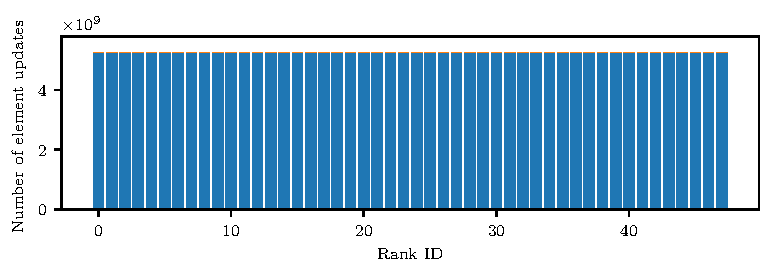
\includegraphics{images/lake_at_rest_uniform_rank_work}}\\
\subfloat[Lake at Rest--Polynomial\label{fig:rb:rank:lar:polynomial}]{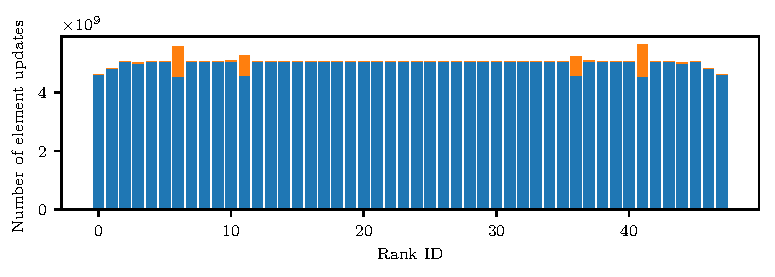
\includegraphics{images/lake_at_rest_polynomial_rank_work}}\\
\subfloat[Carrier-Greenspan--Uniform]{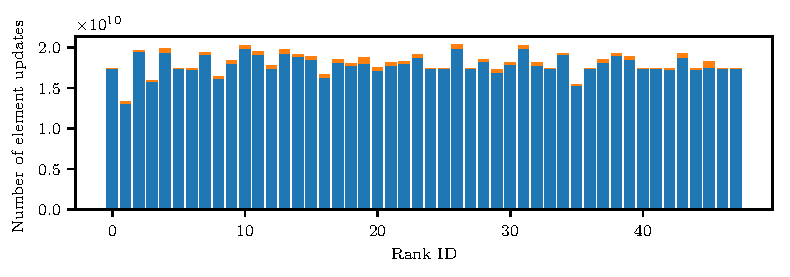
\includegraphics{images/carrier_greenspan_uniform_rank_work}}\\
\subfloat[Carrier-Greenspan--Polynomial]{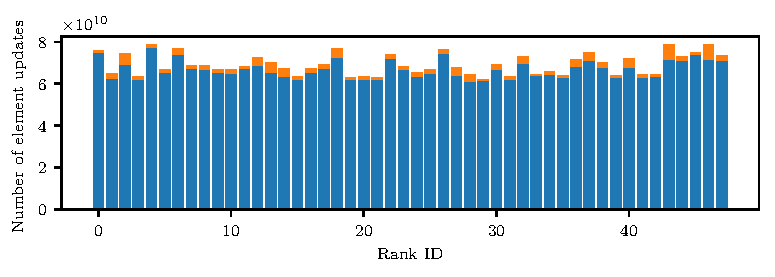
\includegraphics{images/carrier_greenspan_polynomial_rank_work}}
\caption{Cumulative number of element updates committed---shown in \cbox{blueplot}---and rolled back---shown in \cbox{orangeplot} updates for each rank.}
\label{fig:rb:rank}
\end{figure}

In Figure~\ref{fig:rb:rank}, we display the amount of work done by each rank throughout the simulation. The plots show that the load balancing approaches do a reasonable job of balancing committed updates across all ranks. To estimate the impact of rollback on the time to solution, we introduce the time averaged imbalance as
\begin{equation*}
I_C = \frac{1}{T}\int_0^T \frac{ \max_r u_c(r, t) - \overline{u_c}(t)}{\overline{u_c}(t) } \,\mathrm{d} t,
\end{equation*}
where $u_c(r,t)$ is the rate of updates committed on rank $r$ at time $t$, and $\overline{u_c}(t)$ corresponds to the mean number of updates committed at time $t$. We also define the rollback based imbalance as
\begin{equation*}
I_{C+RB} = \frac{1}{T} \int_0^T \frac{ \max_r \left(u_c(r,t) + u_{rb}(r,t) \right)- \overline{u_c}(t)}{\overline{u_c}(t) } \,\mathrm{d} t,
\end{equation*}
where $u_{rb}(r,t)$ corresponds to the rate of updates rolled back on rank $r$. The aim of comparing the two metrics is to identify what percentage of the performance degradation is due to poor load balance versus misspeculation. The update and rollback densities are estimated by calculating how many updates are rolled back or committed every second.
In a strictly performance oriented setting, we do not care about the absolute amount of rollback, but rather only about rollback incurred on the critical path, i.e. most overworked rank. In Table~\ref{tab:rb:imb}, we compare the two imbalances for the test cases. For the Carrier-Greenspan problem, we observe that due to the fact that the actors which are rolled back are distributed across many ranks, rollback does not accumulate on any single rank. We estimate that the time to solution would only be $2\%$ faster if we didn't incur any rollback. On the other hand, for the polynomial lake at rest problem, the rollback is confined to only a few ranks. In turn, these ranks slow down the otherwise well balanced problem configuration. We predict that we would observe a $12\%$ reduction in time to solution if this rollback were not present.

\begin{table}
\centering
\begin{tabular}{|c | c c c c|}
\hline & \multicolumn{2}{c}{Lake at Rest} & \multicolumn{2}{c|}{Carrier-Greenspan} \\
Mesh Type& $I_C$ & $I_{C+RB}$ & $I_C$ & $I_{C+RB}$ \\ \hline
Uniform  & 1.00 & 1.00 & 1.12 & 1.14\\ \hline
Polynomial & 1.01 & 1.13 & 1.16 & 1.18\\ \hline
\end{tabular}
\caption{Time-averaged imbalance with and without rollback}
\label{tab:rb:imb}
\end{table}
\subsubsection*{Justify better why you did not explore conservative event-driven simulation.}

{\it This discussion has been added to p. 100}

\begin{figure}
  \centering
  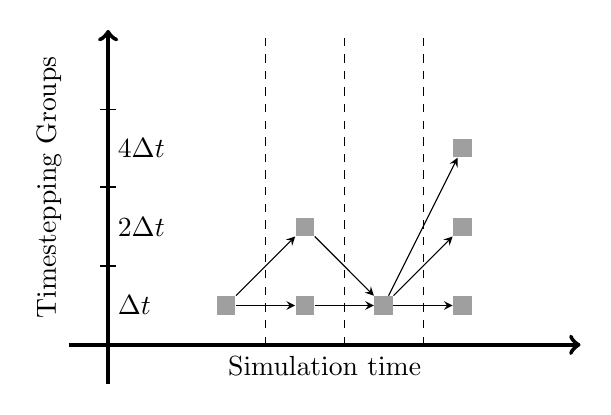
\begin{tikzpicture}
    \draw[->,ultra thick] (-1,-0.5)--(-1,4);
    \node[rotate=90] at (-1.75, 2)  (a) {Timestepping Groups};
\draw[->,ultra thick] (-1.5,0)--(5,0) node[midway,below]{Simulation time};

    \draw[|-|] (-1,0)--(-1,1) node[midway,right] {$\Delta t$};
    \draw[|-|] (-1,1)--(-1,2) node[midway,right] {$2 \Delta t$};
    \draw[|-|] (-1,2)--(-1,3) node[midway,right] {$4 \Delta t$};

\draw[dashed] (1,0)--(1,4);
\draw[dashed] (2,0)--(2,4);
\draw[dashed] (3,0)--(3,4);

\begin{scope}
    \node[fill=darkgray!50] (AI) at (0.5,0.5) {};
    \node[fill=darkgray!50] (AII) at (1.5,0.5) {};
    \node[fill=darkgray!50] (AIII) at (2.5,0.5) {};
    \node[fill=darkgray!50] (AIV) at (3.5,0.5) {};
    \node[fill=darkgray!50] (BI) at (1.5,1.5) {};
    \node[fill=darkgray!50] (BII) at (3.5,1.5) {};
    \node[fill=darkgray!50] (CI) at (3.5,2.5) {};
\end{scope}

\begin{scope}[>=stealth,black]
  \path[->] (AI) edge (AII);
  \path[->] (AI) edge (BI);
  \path[->] (AII) edge (AIII);
  \path[->] (BI) edge (AIII);
  \path[->] (AIII) edge (AIV);
  \path[->] (AIII) edge (BII);
  \path[->] (AIII) edge (CI);
\end{scope}

  \end{tikzpicture}
\caption{Illustration of conservative parallel discrete event simulation with no look ahead.}
\label{fig:cons}
\end{figure}
An alternative way to parallelize the algorithm would be through conservative parallel discrete event simulation. Whereas the timewarp based algorithm has a mechanism to correct causality violations. Conservative parallel discrete event simulation requires the program to guarantee that no causality violation can occur. Perhaps the most simple version of a conservative parallel discrete event simulation would be to maintain a global priority queue and execute events with the lowest timestamp. A schematic of elements updating in various timestepping groups is shown in Figure~\ref{fig:cons}. This implementation suffers from insufficient available parallelism and significant synchronization overhead. For the hurricane storm surge problem considered in~\cite{Dawson2013}, a mesh with $\mathcal{O}(10^6)$ elements only has $\mathcal{O}(10^4)$ elements stepping in the smallest timestepping group. Amdahl's law limits the scalability of any such approach.

Conservative parallel discrete event simulations introduce more parallelism into the system through the introduction of {\em look ahead}. If for a given global timestamp, we can ensure that no causality violations can occur over some time interval, all events scheduled within that interval may be safely executed. The use of a global priority queue corresponds to a look ahead of zero. To derive look ahead estimates for systems of conservation laws, we must prove that no push flux---the result of a neighbor updating---will be processed within the look ahead interval. 

To achieve a viable implementation using a conservative parallel discrete event simulation, two major problems need to be resolved. 
\begin{enumerate}
\item {\em Energy-based look ahead estimates}: The wavespeed $|\Lambda|$ can be bounded above and below by the energy of the system with a constant for Burgers' equation and the shallow water equations. This intuition provides a useful glimpse into the evolution of $\Lambda$. We know from the Burgers' equation example used in the motivation of this chapter that any look ahead estimate must consider the discrete domain of dependence of the problem. This requires global knowledge since pathological spikes of energy could exist anywhere. 
However, a hope would be that once initial global communication has occurred, we may be able to derive estimates for local energy growth, and thus bound changes in wavespeed $|\Lambda|$. By determining the growth of $\Lambda$, look ahead estimates can then be determined by deriving lower bounds on when neighboring actors will update.

\item {\em Loosening of TVD properties}: The aim of this thesis is to derive a total variation diminishing timestepping scheme. The analysis used in this chapter requires that the event trace be locally ordered. From a parallel discrete event standpoint, this is problematic as it may generate event cascades, i.e. events scheduled on neighboring actors with the same timestamp. This complicates the derivation of look ahead estimates, because in addition to bounding the growth of $|\Lambda|$, we also need to ensure that no locally ordering violations can occur. Lastly, the binning of timesteps to powers of two of $\Delta t_{\min}$ also presents issues. Given an actor at timestep 10 with a largest allowable timestep of 15, the next update would occur at 24 (i.e. the largest multiple of 8). If however, at time 10, a message is processed that causes the wavespeed to decrease and the allowable timestep increased to 16, the timestep would occur sooner---rather than later---at time 16 (the largest multiple of 16). Thus, there are also cases where lowering the wavespeed causes the proposed timestep to {\em decrease}. We conjecture that the need for locally ordered event traces can be eliminated by relaxing the requirement of total variation diminishing to total variation bounded. Total variation bounded solutions correspond to a larger, but still stable solution class. The relaxation to total variation bounded solutions may be inevitable as we move to higher order timestepping schemes, e.g.~\cite{Constantinescu2007}. Apart from allowing for easier derivation of look ahead estimates, eliminating the locally ordered event trace requirement would also eliminate the need to bin timesteps, reducing the total amount of work  performed.
\end{enumerate}

Given the difficulties required to obtain meaningful look ahead estimates, we have primarily focused on optimistic speculation in this thesis. Rather than focus on deriving look ahead estimates, we have found it easier to derive tests which identify when speculation is guaranteed to be rolled-back based on local information and then simply wait for the message that causes the rollback of any subsequent events to be processed. Furthermore, given the near optimal performance of the optimistic parallel discrete event simulator for this small problem, we need to identify use cases to motivate development of conservative parallel discrete event simulation.


\subsubsection*{Given an estimate of how much time paritioning.}
{\it The Dynamic load balancing edit is on p. 35. Gurobi partitioning information has been added to p. 91.}
\begin{itemize}
\item {\bf Dynamic Load Balancing:} For the semi-static load balancing approach, note that we are repartitioning the submesh graph rather than the finite element mesh. This decreases the number of vertices in the graphs partitioned by METIS by two to three orders of magnitude. The amount of time spent inside the offloaded thread performing the repartitioning ranges from $700\,\mathrm{ms}$ for the 1200 core simulation up to $3700\,\mathrm{ms}$ for the 6000 core case.

\item {\bf Adaptive Local Timestepping:} The goal of the partitioning scheme outlined in Section 3.5.3 is to minimize the impact of load imbalance by finding the optimal static partitioning scheme.
As a lower bound, we assume that all ranks have the same amount of work throughout the simulation, yielding the following optimal runtime $T^*$,
\begin{equation*}
T^* = \frac{1}{n_{ranks}} \int_0^{t_{end}} \sum_{j=1}^{n_{el}} w_j(\tau) \,\mathrm{d}\tau,
\end{equation*}
where $w_j$ is the work associated with a given cell at a given point in time. The Gurobi partitioning then optimizes $(T - T^*)/T^*$. For both Carrier-Greenspan problems, we let Gurobi run for 6 minutes, and then use the best solution found. There are significant variations in the difficulty of the load balancing the problem. For the uniform mesh, the partitioner returns with a solution with an imbalance of $4\%$. For the solution to the polynomial mesh, Gurobi returns a solution with an imbalance of $25\%$. However, Gurobi also reports that a lower bound on the best possible partitioning is $20\%$ indicating that the solution is within $5\%$ of the optimal partitioning.

We also remark that this load balancing strategy may have limited viability outside of shared memory applications. The partitioning problem does not account for edge cuts, and the generated partitions have more than $97\%$ of edges cut for both meshes.
Additionally the reliance on a good estimate of $w_j$ is not a reasonable assumption. In the case of hurricane storm surge, this knowledge requires an informed guess into when and where flooding occurs, which is precisely the problem we are interested in solving. In practice, dynamic load balancing strategies as outlined in Chapter 2, may be necessary to achieve good resource utilization.
\end{itemize}


\bibliographystyle{plain}
\bibliography{src.bib}
\end{document}